% THIS DOCUMENT IS FOLLOWS THE VOLERE TEMPLATE BY Suzanne Robertson and James Robertson
% ONLY THE SECTION HEADINGS ARE PROVIDED
%
% Initial draft from https://github.com/Dieblich/volere
%
% Risks are removed because they are covered by the Hazard Analysis
\documentclass[12pt]{article}

\usepackage{booktabs}
\usepackage{tabularx}
\usepackage{hyperref}
\usepackage{multicol}
\usepackage[dvipsnames]{xcolor}
\usepackage{enumitem}
\usepackage{tcolorbox}
\usepackage{array}

\hypersetup{
    bookmarks=true,         % show bookmarks bar?
      colorlinks=true,      % false: boxed links; true: colored links
    linkcolor=red,          % color of internal links (change box color with linkbordercolor)
    citecolor=green,        % color of links to bibliography
    filecolor=magenta,      % color of file links
    urlcolor=cyan           % color of external links
}

\newenvironment{myreq}[1]{%
\setlist[description]{font=\normalfont\color{darkgray}}%
\begin{tcolorbox}[colframe=black,colback=white, sharp corners, boxrule=1pt]%
\bfseries\color{blue}%
\begin{description}#1}%
{\end{description}\end{tcolorbox}}

\newcommand{\threeinline}[3]{\begin{multicols}{3}#1 #2 #3\end{multicols}}
\newcommand{\twoinline}[2]{\begin{multicols}{2}#1 #2\end{multicols}}

\newcommand{\reqno}{\item[Requirement \#:]}
\newcommand{\reqtype}{\item[Requirement Type:]}
\newcommand{\reqevent}{\item[Event/BUC/PUC \#:]}
\newcommand{\reqdesc}{\item[Description:]}
\newcommand{\reqrat}{\item[Rationale:]}
\newcommand{\reqorig}{\item[Originator:]}
\newcommand{\reqfit}{\item[Fit Criterion:]}
\newcommand{\reqsatis}{\item[Customer Satisfaction:]}
\newcommand{\reqdissat}{\item[Customer Dissatisfaction:]}
\newcommand{\reqdep}{\item[Dependencies:]}
\newcommand{\reqconf}{\item[Conflicts:]}
\newcommand{\reqmater}{\item[Materials:]}
\newcommand{\reqhist}{\item[History:]}

\newcommand{\lips}{\textit{Insert your content here.}}

%% Comments

\usepackage{color}

\newif\ifcomments\commentstrue %displays comments
%\newif\ifcomments\commentsfalse %so that comments do not display

\ifcomments
\newcommand{\authornote}[3]{\textcolor{#1}{[#3 ---#2]}}
\newcommand{\todo}[1]{\textcolor{red}{[TODO: #1]}}
\else
\newcommand{\authornote}[3]{}
\newcommand{\todo}[1]{}
\fi

\newcommand{\wss}[1]{\authornote{blue}{SS}{#1}} 
\newcommand{\plt}[1]{\authornote{magenta}{TPLT}{#1}} %For explanation of the template
\newcommand{\an}[1]{\authornote{cyan}{Author}{#1}}

%% Common Parts

\newcommand{\progname}{Student Evaluation App} % PUT YOUR PROGRAM NAME HERE
\newcommand{\authname}{Team 29
\\ Nicholas Fabugais-Inaba
\\ Casra Ghazanfari
\\ Alex Verity
\\ Jung Woo Lee} % AUTHOR NAMES                  

\usepackage{hyperref}
    \hypersetup{colorlinks=true, linkcolor=blue, citecolor=blue, filecolor=blue,
                urlcolor=blue, unicode=false}
    \urlstyle{same}
                                


\begin{document}

\title{Software Requirements Specification for \progname: Softball League Scheduling and Management Web Application} 
\author{\authname}
\date{\today}
	
\maketitle

~\newpage

\pagenumbering{roman}

\tableofcontents

~\newpage

\section*{Revision History}

\begin{tabularx}{\textwidth}{p{3cm}p{2cm}X}
\toprule {\textbf{Date}} & {\textbf{Version}} & {\textbf{Notes}}\\
\midrule
October 7, 2024 & 1.0 & TA Feedback\\
October 9, 2024 & 1.1 & Rev0\\
\bottomrule
\end{tabularx}

~\\

~\newpage
\section{Purpose of the Project}

\subsection{User Business}

The McMaster GSA softball league's current scheduling and management platform
is used from the 1st week of May till the last week of August. The website
creates a season schedule based on the 30-40 teams that are entered into the
league by their respective captains. If scheduling conflicts or weather concerns
occur, games are able to be rescheduled by the team captains based on a team's
availability. For the many users interacting with the platform, individuals need
an intuitive interface that is robust and will allow administrators to easily
maintain the system, especially when the website experiences problems. The current
platform lacks the capabilities to provide these functionalities to the players,
captains, and commissioners. With this project, our team is provided an
opportunity to apply our software engineering background to fulfill a
desired need for an upgrade to an outdated website.

\subsection{Goals of the Project}
Our goals with the project are to recreate everything the current website
solution does, with a better user interface and a more stable foundation, so
that future site admins and league commissioners don't have to deal with the
solution breaking or captains/players not understanding how to use the tool.
We also plan to add features such as player accounts to help players view
their schedules, and a standings viewer to see league scores.

\section{Stakeholders}
\subsection{Client}

The client of the project, Dr. Jake Nease, is an active participant in the
McMaster GSA softball league and understands the difficulties associated with
the current scheduling and management platform. The stability and maintainability
concerns with the website are driving factors that contribute to the need for
an improved interface.

\subsection{Customer}

The customers for this project include the players, captains, commissioners,
umpires, and other individuals that may interact with the website. These
individuals require an easy-to-use platform that allows them to seamlessly
enter the website and view the season schedule, whether or not they have an
account created.

\subsection{Other Stakeholders}
\lips
\subsection{Hands-On Users of the Project}
\lips
\subsection{Personas}

\begin{itemize}
  \item [1.]
  
  Josh Brown is a 26 year old player that has recently joined the McMaster GSA
  softball league and he is unfamiliar with how the website functions. As someone
  who understands how technology works though, he is able to navigate the interface
  quite well. However, some links he interacts with give him a 404 page not found
  error. This aggravates Josh as he just wants to understand certain information
  about the softball league, but the website isn't able to provide it to him
  because the links on the website are faulty or other issues occur. Josh, along
  with many others who are new to the league, may be technically literate, but due
  to the structural integrity of the system, there are many times where users may
  not be able to access certain information because there is either an error or a
  link that leads to nothing.

  \item [2.]
  
  Ken Phillips is a 58 year old captain for his McMaster GSA softball team and he has
  been using the current website for as long as he can remember. Although he is not
  too familiar with how technology works, he is still able to navigate and utilize the
  website's functionalities as he has used them for quite some time now. Unfortunately,
  with the creation of the new website, even though the website has the same existing
  functions as the old system, he is not as familiar with how to navigate the interface
  the same way he has before. Ken and other individuals that may be comfortable and
  familiar with the current outdated platform, need the new website to be easy-to-use,
  especially for people that are either older or not as technically literate.

\end{itemize}


\subsection{Priorities Assigned to Users}
\lips
\subsection{User Participation}
\lips
\subsection{Maintenance Users and Service Technicians}
\lips

\section{Mandated Constraints}
\subsection{Solution Constraints}

\begin{myreq}
  \threeinline
    {\reqno 0}
    {\reqtype 0}
    {\reqevent 2,3}
  \reqdesc Non-commissioner accounts can only be a member of one team.
  \reqrat To ensure competition is fair and to avoid captains accidentally
  making extranious teams, users are limited to one team each.
  \reqorig Alex Verity
  \reqfit Once a team is created by a captain or a team is joined by a player,
  they shall not be allowed to use the functionality to create a team or join
  a team.
  \twoinline
    {\reqsatis 2}
    {\reqdissat 2}
  \twoinline
  {\reqdep None}
  {\reqconf None}
  \reqmater
  \reqhist
\end{myreq}

\subsection{Implementation Environment of the Current System}
\lips
\subsection{Partner or Collaborative Applications}
\lips
\subsection{Off-the-Shelf Software}
\lips
\subsection{Anticipated Workplace Environment}
\lips
\subsection{Schedule Constraints}
\lips
\subsection{Budget Constraints}
\lips
\subsection{Enterprise Constraints}
\lips

\section{Naming Conventions and Terminology}
\subsection{Glossary of All Terms, Including Acronyms, Used by Stakeholders
involved in the Project}
Sandlot: Management software for a softball baseball league, the software that
is the subject of this document.\\\\
Player: A person who plays on a baseball team in the league. They have an
account on Sandlot and are a member of a team.\\\\
Captain: A person who plays and leads a baseball team in the league. They are
in charge of defining the team's information on Sandlot.\\\\
Team: A name and a list of players representing a baseball team defined by a
captain. Teams are stored on a database on Sandlot.\\\\

\section{Relevant Facts And Assumptions}
\subsection{Relevant Facts}
\begin{itemize}
  \item The current solution is a website with url 
  \url{https://www.gsasoftball.ca/}
  \item There are currently 25-32 teams in the league playing an average of
  100 games a month.
  \item Many users are older and require an intuitive UI to enjoy using the
  site
\end{itemize}

\subsection{Business Rules}
Not applicable

\subsection{Assumptions}
\begin{itemize}
  \item All users will understand how to log in to a website using a username
  and password.
\end{itemize}

\section{The Scope of the Work}
\subsection{The Current Situation}
It is important to note that we will not be using the existing solution other
than as a feature guide. The current solution is hosted on the web and is
written in PHP. The current login system does not use a username and password.
Only captains can log in, and they are emailed an ASCII code which they use to
access the website to schedule games and submit scores. Commissioners can login
in the same way as captains and can modify schedules, scores and team
compositions as needed. Currently the standings functionality, which would
allow users to view the scores of played games, is not working.
\subsection{The Context of the Work}
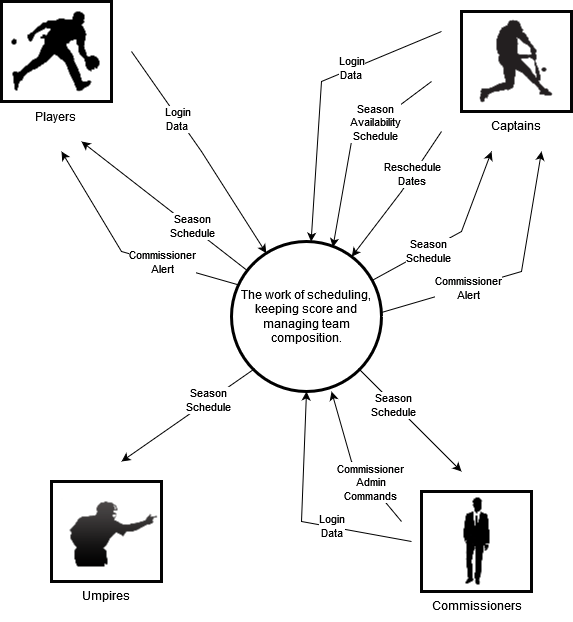
\includegraphics[scale=0.6]{6b_context_diagram.png}
\subsection{Work Partitioning}
  \begin{center}
    \begin{tabular}{|m{4cm}|m{4cm}|m{6cm}|}
      \hline
      Event Name & Input and Output & Summary of BUC\\
      \hline
      1. User logs in & Login Data (in) & A player, captain or commissioner
      enters their username and password and the system grants them access to
      their account.\\
      2. Captain creates a team & New Team Information (in) & At the
      start of the season, captains can enter team information such as a team
      name. This registers a new team.\\
      3. Player requests to join a team & Team Join Request (in) & At the
      start of the season, players are not assigned to a team and must request
      to join one.\\
      4. Season starts and availability entered & Season Availability Schedule
      (in) & Record the team captain's entered availability schedule. This
      will be used to generate the league schedule.\\
      5. Reschedule request entered & Reschedule Dates (in) & Record
      availability dates the requesting captain entered as alternates for the
      planned date.\\
      6. Reschedule request recieved & Reschedule Dates (out) & Send the dates
      the captain who sent the request submit to the other team's captain.\\
      7. User navigates to schedule section & Season Schedule (out) & Display
      stored season schedule (if available) to site user.\\
      8. User submits alert & Alert Content (in) & Commissioners can submit
      customalerts to send to any chosen users.\\
      9. System sends alert & Alert Content (out) & Send the alert to any user
      the alert must reach.\\
      10. Commissioner inputs admin command & Commissioner Admin Commands (in)
      & Commissioners have the ability to overwrite team composition and
      schedule.\\
      \hline
    \end{tabular}
  \end{center}
\subsection{Specifying a Business Use Case (BUC)}
\lips

\section{Business Data Model and Data Dictionary}
\subsection{Business Data Model}
\lips
\subsection{Data Dictionary}
\lips

\section{The Scope of the Product}
\subsection{Product Boundary}
\lips
\subsection{Product Use Case Table}
\lips
\subsection{Individual Product Use Cases (PUC's)}
\lips

\section{Functional Requirements}
\subsection{Functional Requirements}

\begin{myreq}
  \threeinline
    {\reqno 75}
    {\reqtype 9}
    {\reqevent 7.9}
  \reqdesc description text description text description text 
  \reqrat some more text some more text some more text 
  \reqorig other text other text other text 
  \reqfit longer text that needs more than one line longer text that needs more than one line
  \twoinline
    {\reqsatis 5}
    {\reqdissat 3}
  \twoinline
  {\reqdep some more text}
  {\reqconf 111}
  \reqmater other text other text other text 
  \reqhist other text other text other text 
\end{myreq}

\begin{myreq}
  \threeinline
    {\reqno 1}
    {\reqtype 0}
    {\reqevent 7}
  \reqdesc System must display the season schedule and standings to all users
  without login.
  \reqrat Users who don't have a login (ie. spectators and umpires) will still
  need to access the schedule and standings, so it should be visible to all.
  \reqorig Alex Verity
  \reqfit The schedule and standings shall be viewable without entering a
  username and password.
  \twoinline
    {\reqsatis 3}
    {\reqdissat 3}
  \twoinline
  {\reqdep None}
  {\reqconf None}
  \reqmater
  \reqhist
\end{myreq}

\begin{myreq}
  \threeinline
    {\reqno 2}
    {\reqtype 0}
    {\reqevent 2}
  \reqdesc Captains should be able to create a team which is added to the
  Sandlot database.
  \reqrat Teams are defined by captains, in charge of scheduling and
  recording scores. Captains must be able to define teams at the start of the
  season.
  \reqorig Alex Verity
  \reqfit When captains make a team, it should be added to the Sandlot
  database.
  \twoinline
    {\reqsatis 5}
    {\reqdissat 5}
  \twoinline
  {\reqdep None}
  {\reqconf None}
  \reqmater
  \reqhist
\end{myreq}

\section{Look and Feel Requirements}
\subsection{Appearance Requirements}
\lips
\subsection{Style Requirements}
\lips

\section{Usability and Humanity Requirements}
\subsection{Ease of Use Requirements}
\lips
\subsection{Personalization and Internationalization Requirements}
\lips
\subsection{Learning Requirements}
\lips
\subsection{Understandability and Politeness Requirements}
\lips
\subsection{Accessibility Requirements}
\lips

\section{Performance Requirements}
\subsection{Speed and Latency Requirements}
\lips
\subsection{Safety-Critical Requirements}
\lips
\subsection{Precision or Accuracy Requirements}
\lips
\subsection{Robustness or Fault-Tolerance Requirements}
\lips
\subsection{Capacity Requirements}
\lips
\subsection{Scalability or Extensibility Requirements}
\lips
\subsection{Longevity Requirements}
\lips

\section{Operational and Environmental Requirements}
\subsection{Expected Physical Environment}
\lips
\subsection{Wider Environment Requirements}
\lips
\subsection{Requirements for Interfacing with Adjacent Systems}
\lips
\subsection{Productization Requirements}
\lips
\subsection{Release Requirements}
\lips

\section{Maintainability and Support Requirements}
\subsection{Maintenance Requirements}
\lips
\subsection{Supportability Requirements}
\lips
\subsection{Adaptability Requirements}
\lips

\section{Security Requirements}
\subsection{Access Requirements}
\lips
\subsection{Integrity Requirements}
\lips
\subsection{Privacy Requirements}
\lips
\subsection{Audit Requirements}
\lips
\subsection{Immunity Requirements}
\lips

\section{Cultural Requirements}
\subsection{Cultural Requirements}
\lips

\section{Compliance Requirements}
\subsection{Legal Requirements}
\lips
\subsection{Standards Compliance Requirements}
\lips

\section{Open Issues}
\lips

\section{Off-the-Shelf Solutions}
\subsection{Ready-Made Products}
\lips
\subsection{Reusable Components}
\lips
\subsection{Products That Can Be Copied}
\lips

\section{New Problems}
\subsection{Effects on the Current Environment}
\lips
\subsection{Effects on the Installed Systems}
\lips
\subsection{Potential User Problems}
\lips
\subsection{Limitations in the Anticipated Implementation Environment That May
Inhibit the New Product}
\lips
\subsection{Follow-Up Problems}
\lips

\section{Tasks}
\subsection{Project Planning}
\lips
\subsection{Planning of the Development Phases}
\lips

\section{Migration to the New Product}
\subsection{Requirements for Migration to the New Product}
\lips
\subsection{Data That Has to be Modified or Translated for the New System}
\lips

\section{Costs}
\lips
\section{User Documentation and Training}
\subsection{User Documentation Requirements}
\lips
\subsection{Training Requirements}
\lips

\section{Waiting Room}
\lips

\section{Ideas for Solution}
\lips

\newpage{}
\section*{Appendix --- Reflection}

The information in this section will be used to evaluate the team members on the
graduate attribute of Lifelong Learning.  Please answer the following questions:

\begin{enumerate}
  \item What knowledge and skills will the team collectively need to acquire to
  successfully complete this capstone project?  Examples of possible knowledge
  to acquire include domain specific knowledge from the domain of your
  application, or software engineering knowledge, mechatronics knowledge or
  computer science knowledge.  Skills may be related to technology, or writing,
  or presentation, or team management, etc.  You should look to identify at
  least one item for each team member.
  \item For each of the knowledge areas and skills identified in the previous
  question, what are at least two approaches to acquiring the knowledge or
  mastering the skill?  Of the identified approaches, which will each team
  member pursue, and why did they make this choice?
\end{enumerate}

\end{document}